\documentclass[twoside]{book}

% Packages required by doxygen
\usepackage{fixltx2e}
\usepackage{calc}
\usepackage{doxygen}
\usepackage[export]{adjustbox} % also loads graphicx
\usepackage{graphicx}
\usepackage[utf8]{inputenc}
\usepackage{makeidx}
\usepackage{multicol}
\usepackage{multirow}
\PassOptionsToPackage{warn}{textcomp}
\usepackage{textcomp}
\usepackage[nointegrals]{wasysym}
\usepackage[table]{xcolor}

% Font selection
\usepackage[T1]{fontenc}
\usepackage[scaled=.90]{helvet}
\usepackage{courier}
\usepackage{amssymb}
\usepackage{sectsty}
\renewcommand{\familydefault}{\sfdefault}
\allsectionsfont{%
  \fontseries{bc}\selectfont%
  \color{darkgray}%
}
\renewcommand{\DoxyLabelFont}{%
  \fontseries{bc}\selectfont%
  \color{darkgray}%
}
\newcommand{\+}{\discretionary{\mbox{\scriptsize$\hookleftarrow$}}{}{}}

% Page & text layout
\usepackage{geometry}
\geometry{%
  a4paper,%
  top=2.5cm,%
  bottom=2.5cm,%
  left=2.5cm,%
  right=2.5cm%
}
\tolerance=750
\hfuzz=15pt
\hbadness=750
\setlength{\emergencystretch}{15pt}
\setlength{\parindent}{0cm}
\setlength{\parskip}{3ex plus 2ex minus 2ex}
\makeatletter
\renewcommand{\paragraph}{%
  \@startsection{paragraph}{4}{0ex}{-1.0ex}{1.0ex}{%
    \normalfont\normalsize\bfseries\SS@parafont%
  }%
}
\renewcommand{\subparagraph}{%
  \@startsection{subparagraph}{5}{0ex}{-1.0ex}{1.0ex}{%
    \normalfont\normalsize\bfseries\SS@subparafont%
  }%
}
\makeatother

% Headers & footers
\usepackage{fancyhdr}
\pagestyle{fancyplain}
\fancyhead[LE]{\fancyplain{}{\bfseries\thepage}}
\fancyhead[CE]{\fancyplain{}{}}
\fancyhead[RE]{\fancyplain{}{\bfseries\leftmark}}
\fancyhead[LO]{\fancyplain{}{\bfseries\rightmark}}
\fancyhead[CO]{\fancyplain{}{}}
\fancyhead[RO]{\fancyplain{}{\bfseries\thepage}}
\fancyfoot[LE]{\fancyplain{}{}}
\fancyfoot[CE]{\fancyplain{}{}}
\fancyfoot[RE]{\fancyplain{}{\bfseries\scriptsize Generated by Doxygen }}
\fancyfoot[LO]{\fancyplain{}{\bfseries\scriptsize Generated by Doxygen }}
\fancyfoot[CO]{\fancyplain{}{}}
\fancyfoot[RO]{\fancyplain{}{}}
\renewcommand{\footrulewidth}{0.4pt}
\renewcommand{\chaptermark}[1]{%
  \markboth{#1}{}%
}
\renewcommand{\sectionmark}[1]{%
  \markright{\thesection\ #1}%
}

% Indices & bibliography
\usepackage{natbib}
\usepackage[titles]{tocloft}
\setcounter{tocdepth}{3}
\setcounter{secnumdepth}{5}
\makeindex

% Hyperlinks (required, but should be loaded last)
\usepackage{ifpdf}
\ifpdf
  \usepackage[pdftex,pagebackref=true]{hyperref}
\else
  \usepackage[ps2pdf,pagebackref=true]{hyperref}
\fi
\hypersetup{%
  colorlinks=true,%
  linkcolor=blue,%
  citecolor=blue,%
  unicode%
}

% Custom commands
\newcommand{\clearemptydoublepage}{%
  \newpage{\pagestyle{empty}\cleardoublepage}%
}

\usepackage{caption}
\captionsetup{labelsep=space,justification=centering,font={bf},singlelinecheck=off,skip=4pt,position=top}

%===== C O N T E N T S =====

\begin{document}

% Titlepage & ToC
\hypersetup{pageanchor=false,
             bookmarksnumbered=true,
             pdfencoding=unicode
            }
\pagenumbering{alph}
\begin{titlepage}
\vspace*{7cm}
\begin{center}%
{\Large Doxygen Testing }\\
\vspace*{1cm}
{\large Generated by Doxygen 1.8.13}\\
\end{center}
\end{titlepage}
\clearemptydoublepage
\pagenumbering{roman}
\tableofcontents
\clearemptydoublepage
\pagenumbering{arabic}
\hypersetup{pageanchor=true}

%--- Begin generated contents ---
\chapter{Employee Program (Doxygen Toolkit)}
\label{md_README}
\Hypertarget{md_README}
Author\+: Connor Walsh Date\+: 11/07/2022

This program is designed to store and calculate information relating to employees at a company including Supervisors and Officers. \hyperlink{classEmployee}{Employee}, \hyperlink{classSupervisor}{Supervisor}, and \hyperlink{classOfficer}{Officer} objects can be declared in the main and all of their respective methods can be called on them in order to preform various functions including calculations for pay and related information.

\subsection*{How to Run}


\begin{DoxyItemize}
\item Type \char`\"{}make\char`\"{} to compile the program.
\item Type ./employee to run the executable created by the compilation process.
\item Type \char`\"{}make clean\char`\"{} to delete unwanted files created by the compilation process.
\item When the executable is run, the information currently held in the main is printed. 
\end{DoxyItemize}
\chapter{Hierarchical Index}
\section{Class Hierarchy}
This inheritance list is sorted roughly, but not completely, alphabetically\+:\begin{DoxyCompactList}
\item \contentsline{section}{Employee}{\pageref{classEmployee}}{}
\begin{DoxyCompactList}
\item \contentsline{section}{Officer}{\pageref{classOfficer}}{}
\item \contentsline{section}{Supervisor}{\pageref{classSupervisor}}{}
\end{DoxyCompactList}
\end{DoxyCompactList}

\chapter{Class Index}
\section{Class List}
Here are the classes, structs, unions and interfaces with brief descriptions\+:\begin{DoxyCompactList}
\item\contentsline{section}{\hyperlink{classEmployee}{Employee} \\*This is an \hyperlink{classEmployee}{Employee} object class }{\pageref{classEmployee}}{}
\item\contentsline{section}{\hyperlink{classOfficer}{Officer} \\*Class for an \hyperlink{classOfficer}{Officer} object }{\pageref{classOfficer}}{}
\item\contentsline{section}{\hyperlink{classSupervisor}{Supervisor} \\*This class contains methods to store values for various \hyperlink{classSupervisor}{Supervisor} attributes }{\pageref{classSupervisor}}{}
\end{DoxyCompactList}

\chapter{File Index}
\section{File List}
Here is a list of all documented files with brief descriptions\+:\begin{DoxyCompactList}
\item\contentsline{section}{\hyperlink{Employee_8cpp}{Employee.\+cpp} \\*Implementation of the \hyperlink{classEmployee}{Employee} class }{\pageref{Employee_8cpp}}{}
\item\contentsline{section}{\hyperlink{Employee_8h}{Employee.\+h} \\*\hyperlink{classEmployee}{Employee} header file }{\pageref{Employee_8h}}{}
\item\contentsline{section}{\hyperlink{main_8cpp}{main.\+cpp} \\*Driver for the employee, supervisor, and officer classes }{\pageref{main_8cpp}}{}
\item\contentsline{section}{\hyperlink{Officer_8cpp}{Officer.\+cpp} \\*Implementation of the \hyperlink{classOfficer}{Officer} class }{\pageref{Officer_8cpp}}{}
\item\contentsline{section}{\hyperlink{Officer_8h}{Officer.\+h} \\*Header file for the officer class }{\pageref{Officer_8h}}{}
\item\contentsline{section}{\hyperlink{Supervisor_8cpp}{Supervisor.\+cpp} \\*Implementation of the \hyperlink{classSupervisor}{Supervisor} class }{\pageref{Supervisor_8cpp}}{}
\item\contentsline{section}{\hyperlink{Supervisor_8h}{Supervisor.\+h} \\*\hyperlink{classSupervisor}{Supervisor} header file }{\pageref{Supervisor_8h}}{}
\end{DoxyCompactList}

\chapter{Class Documentation}
\hypertarget{classEmployee}{}\section{Employee Class Reference}
\label{classEmployee}\index{Employee@{Employee}}


This is an \hyperlink{classEmployee}{Employee} object class.  




{\ttfamily \#include \char`\"{}doxygen/\+Employee.\+h\char`\"{}}



Inheritance diagram for Employee\+:\nopagebreak
\begin{figure}[H]
\begin{center}
\leavevmode
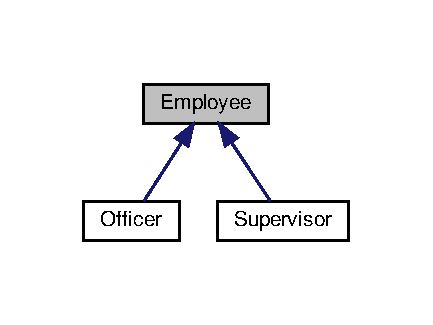
\includegraphics[width=208pt]{classEmployee__inherit__graph}
\end{center}
\end{figure}
\subsection*{Public Member Functions}
\begin{DoxyCompactItemize}
\item 
virtual void \hyperlink{classEmployee_a79556ad700627dba88049f487a34a762}{print} ()
\item 
virtual double \hyperlink{classEmployee_a01c2c44e15434237db28832f6972e960}{calculate\+Pay} ()
\item 
void \hyperlink{classEmployee_a67c345031cf63f515fb09dc675dee5f3}{anniversary} ()
\item 
\hyperlink{classEmployee_a003c7bd08c40924e381eb0750cbb906f}{Employee} ()
\item 
\hyperlink{classEmployee_ad0c935ef9a290a82dcf7865172c90148}{Employee} (int ID, int years, double hourly\+Rate, float hours\+Worked)
\end{DoxyCompactItemize}
\subsection*{Protected Attributes}
\begin{DoxyCompactItemize}
\item 
\mbox{\Hypertarget{classEmployee_ac31134abb9b4004fc015e51ef579b069}\label{classEmployee_ac31134abb9b4004fc015e51ef579b069}} 
double {\bfseries hourly\+Rate}
\item 
\mbox{\Hypertarget{classEmployee_afde35c73d02eb1cfe89e23a80998b42e}\label{classEmployee_afde35c73d02eb1cfe89e23a80998b42e}} 
float {\bfseries hours\+Worked}
\end{DoxyCompactItemize}
\subsection*{Private Attributes}
\begin{DoxyCompactItemize}
\item 
\mbox{\Hypertarget{classEmployee_a832bbae4ee8a704b917f82c4d497bbac}\label{classEmployee_a832bbae4ee8a704b917f82c4d497bbac}} 
int {\bfseries ID}
\item 
\mbox{\Hypertarget{classEmployee_a3e4862d9dfc73becb459a562fa2e25f5}\label{classEmployee_a3e4862d9dfc73becb459a562fa2e25f5}} 
int {\bfseries years}
\end{DoxyCompactItemize}


\subsection{Detailed Description}
This is an \hyperlink{classEmployee}{Employee} object class. 

This class creates an \hyperlink{classEmployee}{Employee} object along with several values relating to employees. 

\subsection{Constructor \& Destructor Documentation}
\mbox{\Hypertarget{classEmployee_a003c7bd08c40924e381eb0750cbb906f}\label{classEmployee_a003c7bd08c40924e381eb0750cbb906f}} 
\index{Employee@{Employee}!Employee@{Employee}}
\index{Employee@{Employee}!Employee@{Employee}}
\subsubsection{\texorpdfstring{Employee()}{Employee()}\hspace{0.1cm}{\footnotesize\ttfamily [1/2]}}
{\footnotesize\ttfamily Employee\+::\+Employee (\begin{DoxyParamCaption}{ }\end{DoxyParamCaption})}

This is the constructor for the \hyperlink{classEmployee}{Employee} class.

\begin{DoxyPrecond}{Precondition}
An \hyperlink{classEmployee}{Employee} object must be declared. 
\end{DoxyPrecond}
\begin{DoxyPostcond}{Postcondition}
An \hyperlink{classEmployee}{Employee} object has been created. 
\end{DoxyPostcond}
\mbox{\Hypertarget{classEmployee_ad0c935ef9a290a82dcf7865172c90148}\label{classEmployee_ad0c935ef9a290a82dcf7865172c90148}} 
\index{Employee@{Employee}!Employee@{Employee}}
\index{Employee@{Employee}!Employee@{Employee}}
\subsubsection{\texorpdfstring{Employee()}{Employee()}\hspace{0.1cm}{\footnotesize\ttfamily [2/2]}}
{\footnotesize\ttfamily Employee\+::\+Employee (\begin{DoxyParamCaption}\item[{int}]{ID,  }\item[{int}]{years,  }\item[{double}]{hourly\+Rate,  }\item[{float}]{hours\+Worked }\end{DoxyParamCaption})}

This is a parameterized constructor for an \hyperlink{classEmployee}{Employee} object.


\begin{DoxyParams}{Parameters}
{\em int} & ID This is the ID for an employee. \\
\hline
{\em int} & years Number of years worked for an employee. \\
\hline
{\em double} & hourly\+Rate Payment per hour for an employee. \\
\hline
{\em float} & hours\+Worked Number of hours worked for an \hyperlink{classEmployee}{Employee}. \\
\hline
\end{DoxyParams}
\begin{DoxyPrecond}{Precondition}
A valid \hyperlink{classEmployee}{Employee} object with valid parameters must be declared. 
\end{DoxyPrecond}
\begin{DoxyPostcond}{Postcondition}
The \hyperlink{classEmployee}{Employee} object has been constructed. 
\end{DoxyPostcond}


\subsection{Member Function Documentation}
\mbox{\Hypertarget{classEmployee_a67c345031cf63f515fb09dc675dee5f3}\label{classEmployee_a67c345031cf63f515fb09dc675dee5f3}} 
\index{Employee@{Employee}!anniversary@{anniversary}}
\index{anniversary@{anniversary}!Employee@{Employee}}
\subsubsection{\texorpdfstring{anniversary()}{anniversary()}}
{\footnotesize\ttfamily void Employee\+::anniversary (\begin{DoxyParamCaption}{ }\end{DoxyParamCaption})}

This function prints the ID for an employee along with their years worked. It also increases the year value by one and changes the hourly\+Rate.

\begin{DoxyPrecond}{Precondition}
An \hyperlink{classEmployee}{Employee} object must be declared by the user. 
\end{DoxyPrecond}
\begin{DoxyReturn}{Returns}
void This function returns nothing. 
\end{DoxyReturn}
\begin{DoxyPostcond}{Postcondition}
Information for the \hyperlink{classEmployee}{Employee} and their years worked has been printed. 
\end{DoxyPostcond}
\mbox{\Hypertarget{classEmployee_a01c2c44e15434237db28832f6972e960}\label{classEmployee_a01c2c44e15434237db28832f6972e960}} 
\index{Employee@{Employee}!calculate\+Pay@{calculate\+Pay}}
\index{calculate\+Pay@{calculate\+Pay}!Employee@{Employee}}
\subsubsection{\texorpdfstring{calculate\+Pay()}{calculatePay()}}
{\footnotesize\ttfamily double Employee\+::calculate\+Pay (\begin{DoxyParamCaption}{ }\end{DoxyParamCaption})\hspace{0.3cm}{\ttfamily [virtual]}}

This method calculates the pay for an employee.

\begin{DoxyPrecond}{Precondition}
An \hyperlink{classEmployee}{Employee} object must be declared before use. 
\end{DoxyPrecond}
\begin{DoxyReturn}{Returns}
double This method returns a double amount for payment. 
\end{DoxyReturn}
\begin{DoxyPostcond}{Postcondition}
The pay for the employee has been calculated. 
\end{DoxyPostcond}


Reimplemented in \hyperlink{classSupervisor_aa37daa89523c08b84ae8141299e036f8}{Supervisor}, and \hyperlink{classOfficer_a1fa1aad39b9e95be7a088990ebf17059}{Officer}.



Referenced by Supervisor\+::calculate\+Pay().

\mbox{\Hypertarget{classEmployee_a79556ad700627dba88049f487a34a762}\label{classEmployee_a79556ad700627dba88049f487a34a762}} 
\index{Employee@{Employee}!print@{print}}
\index{print@{print}!Employee@{Employee}}
\subsubsection{\texorpdfstring{print()}{print()}}
{\footnotesize\ttfamily void Employee\+::print (\begin{DoxyParamCaption}{ }\end{DoxyParamCaption})\hspace{0.3cm}{\ttfamily [virtual]}}

This method prints the values associated with the \hyperlink{classEmployee}{Employee} object.

\begin{DoxyPrecond}{Precondition}
There must be an \hyperlink{classEmployee}{Employee} object to print values from. 
\end{DoxyPrecond}
\begin{DoxyReturn}{Returns}
void This method returns nothing. 
\end{DoxyReturn}
\begin{DoxyPostcond}{Postcondition}
The values in the \hyperlink{classEmployee}{Employee} object have been printed. 
\end{DoxyPostcond}


Reimplemented in \hyperlink{classOfficer_aeadece05a1a0b7fb29bd412830d2e07a}{Officer}, and \hyperlink{classSupervisor_a92483dc9a54904d79b46c6ec4efb3f54}{Supervisor}.



Referenced by Officer\+::print(), and Supervisor\+::print().



The documentation for this class was generated from the following files\+:\begin{DoxyCompactItemize}
\item 
\hyperlink{Employee_8h}{Employee.\+h}\item 
\hyperlink{Employee_8cpp}{Employee.\+cpp}\end{DoxyCompactItemize}

\hypertarget{classOfficer}{}\section{Officer Class Reference}
\label{classOfficer}\index{Officer@{Officer}}


class for an \hyperlink{classOfficer}{Officer} object  




{\ttfamily \#include \char`\"{}doxygen/\+Officer.\+h\char`\"{}}



Inheritance diagram for Officer\+:\nopagebreak
\begin{figure}[H]
\begin{center}
\leavevmode
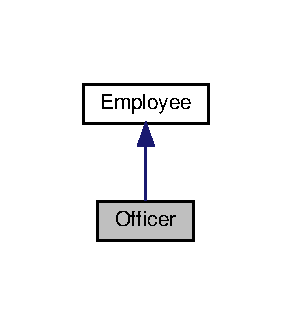
\includegraphics[width=140pt]{classOfficer__inherit__graph}
\end{center}
\end{figure}


Collaboration diagram for Officer\+:\nopagebreak
\begin{figure}[H]
\begin{center}
\leavevmode
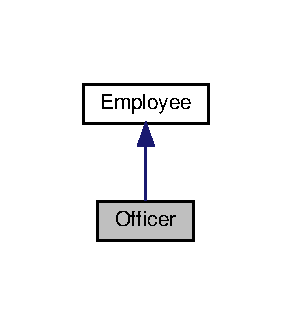
\includegraphics[width=140pt]{classOfficer__coll__graph}
\end{center}
\end{figure}
\subsection*{Public Member Functions}
\begin{DoxyCompactItemize}
\item 
void \hyperlink{classOfficer_aeadece05a1a0b7fb29bd412830d2e07a}{print} ()
\item 
double \hyperlink{classOfficer_a1fa1aad39b9e95be7a088990ebf17059}{calculate\+Pay} ()
\item 
\hyperlink{classOfficer_a80ac1e36a3f36c3a7e12b5dc9320ad89}{Officer} ()
\item 
\hyperlink{classOfficer_ac75c45d6e8628606278cb4ce6596f67f}{Officer} (int ID, int years, double hourly\+Rate, float hours\+Worked, double evilness)
\end{DoxyCompactItemize}
\subsection*{Private Attributes}
\begin{DoxyCompactItemize}
\item 
\mbox{\Hypertarget{classOfficer_a63465c5f16e8148e5bc0a3bb4ecd1781}\label{classOfficer_a63465c5f16e8148e5bc0a3bb4ecd1781}} 
double {\bfseries evilness}
\end{DoxyCompactItemize}
\subsection*{Additional Inherited Members}


\subsection{Detailed Description}
class for an \hyperlink{classOfficer}{Officer} object 

This class creates and then stores various information inside of an \hyperlink{classOfficer}{Officer} object 

\subsection{Constructor \& Destructor Documentation}
\mbox{\Hypertarget{classOfficer_a80ac1e36a3f36c3a7e12b5dc9320ad89}\label{classOfficer_a80ac1e36a3f36c3a7e12b5dc9320ad89}} 
\index{Officer@{Officer}!Officer@{Officer}}
\index{Officer@{Officer}!Officer@{Officer}}
\subsubsection{\texorpdfstring{Officer()}{Officer()}\hspace{0.1cm}{\footnotesize\ttfamily [1/2]}}
{\footnotesize\ttfamily Officer\+::\+Officer (\begin{DoxyParamCaption}{ }\end{DoxyParamCaption})}

This is the Constructor for the \hyperlink{classOfficer}{Officer} class.

\begin{DoxyPrecond}{Precondition}
an \hyperlink{classOfficer}{Officer} object must be declared 
\end{DoxyPrecond}
\begin{DoxyPostcond}{Postcondition}
an \hyperlink{classOfficer}{Officer} object has been constructed 
\end{DoxyPostcond}
\mbox{\Hypertarget{classOfficer_ac75c45d6e8628606278cb4ce6596f67f}\label{classOfficer_ac75c45d6e8628606278cb4ce6596f67f}} 
\index{Officer@{Officer}!Officer@{Officer}}
\index{Officer@{Officer}!Officer@{Officer}}
\subsubsection{\texorpdfstring{Officer()}{Officer()}\hspace{0.1cm}{\footnotesize\ttfamily [2/2]}}
{\footnotesize\ttfamily Officer\+::\+Officer (\begin{DoxyParamCaption}\item[{int}]{ID,  }\item[{int}]{years,  }\item[{double}]{hourly\+Rate,  }\item[{float}]{hours\+Worked,  }\item[{double}]{evilness }\end{DoxyParamCaption})}

This is a parameterized constructor.


\begin{DoxyParams}{Parameters}
{\em int} & ID ID number for an officer \\
\hline
{\em int} & years Years worked at the company \\
\hline
{\em double} & hourly\+Rate amount of pay per hour \\
\hline
{\em float} & hours\+Worked number of hours worked \\
\hline
{\em double} & evilness evil value \\
\hline
\end{DoxyParams}
\begin{DoxyPrecond}{Precondition}
There must be an \hyperlink{classOfficer}{Officer} object declared. 
\end{DoxyPrecond}
\begin{DoxyPostcond}{Postcondition}
An \hyperlink{classOfficer}{Officer} object with the specified parameters has been created. 
\end{DoxyPostcond}


\subsection{Member Function Documentation}
\mbox{\Hypertarget{classOfficer_a1fa1aad39b9e95be7a088990ebf17059}\label{classOfficer_a1fa1aad39b9e95be7a088990ebf17059}} 
\index{Officer@{Officer}!calculate\+Pay@{calculate\+Pay}}
\index{calculate\+Pay@{calculate\+Pay}!Officer@{Officer}}
\subsubsection{\texorpdfstring{calculate\+Pay()}{calculatePay()}}
{\footnotesize\ttfamily double Officer\+::calculate\+Pay (\begin{DoxyParamCaption}{ }\end{DoxyParamCaption})\hspace{0.3cm}{\ttfamily [virtual]}}

This method calculates the pay for an employee.

\begin{DoxyPrecond}{Precondition}
An \hyperlink{classEmployee}{Employee} object must be declared before use. 
\end{DoxyPrecond}
\begin{DoxyReturn}{Returns}
double This method returns a double amount for payment. 
\end{DoxyReturn}
\begin{DoxyPostcond}{Postcondition}
The pay for the employee has been calculated. 
\end{DoxyPostcond}


Reimplemented from \hyperlink{classEmployee_a01c2c44e15434237db28832f6972e960}{Employee}.

\mbox{\Hypertarget{classOfficer_aeadece05a1a0b7fb29bd412830d2e07a}\label{classOfficer_aeadece05a1a0b7fb29bd412830d2e07a}} 
\index{Officer@{Officer}!print@{print}}
\index{print@{print}!Officer@{Officer}}
\subsubsection{\texorpdfstring{print()}{print()}}
{\footnotesize\ttfamily void Officer\+::print (\begin{DoxyParamCaption}{ }\end{DoxyParamCaption})\hspace{0.3cm}{\ttfamily [virtual]}}

This method prints the \hyperlink{classOfficer}{Officer} object information.

\begin{DoxyPrecond}{Precondition}
There must be an \hyperlink{classOfficer}{Officer} object declared. 
\end{DoxyPrecond}
\begin{DoxyReturn}{Returns}
void This method returns nothing. 
\end{DoxyReturn}
\begin{DoxyPostcond}{Postcondition}
The \hyperlink{classOfficer}{Officer} information has been printed. 
\end{DoxyPostcond}


Reimplemented from \hyperlink{classEmployee_a79556ad700627dba88049f487a34a762}{Employee}.



The documentation for this class was generated from the following files\+:\begin{DoxyCompactItemize}
\item 
\hyperlink{Officer_8h}{Officer.\+h}\item 
\hyperlink{Officer_8cpp}{Officer.\+cpp}\end{DoxyCompactItemize}

\hypertarget{classSupervisor}{}\section{Supervisor Class Reference}
\label{classSupervisor}\index{Supervisor@{Supervisor}}


This class contains methods to store values for various \hyperlink{classSupervisor}{Supervisor} attributes.  




{\ttfamily \#include \char`\"{}doxygen/\+Supervisor.\+h\char`\"{}}



Inheritance diagram for Supervisor\+:\nopagebreak
\begin{figure}[H]
\begin{center}
\leavevmode
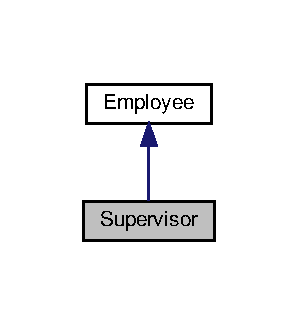
\includegraphics[width=143pt]{classSupervisor__inherit__graph}
\end{center}
\end{figure}


Collaboration diagram for Supervisor\+:\nopagebreak
\begin{figure}[H]
\begin{center}
\leavevmode
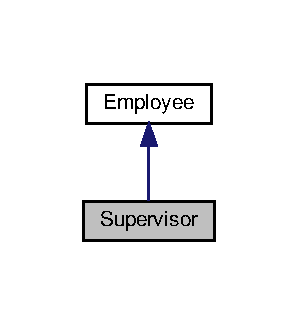
\includegraphics[width=143pt]{classSupervisor__coll__graph}
\end{center}
\end{figure}
\subsection*{Public Member Functions}
\begin{DoxyCompactItemize}
\item 
void \hyperlink{classSupervisor_a92483dc9a54904d79b46c6ec4efb3f54}{print} ()
\item 
double \hyperlink{classSupervisor_aa37daa89523c08b84ae8141299e036f8}{calculate\+Pay} ()
\item 
\hyperlink{classSupervisor_a9d7eafc36b5429092ba0f758bc7841c4}{Supervisor} ()
\item 
\hyperlink{classSupervisor_a02d9245744652deb20e9408001d6ed3b}{Supervisor} (int ID, int years, double hourly\+Rate, float hours\+Worked, int num\+Supervised)
\end{DoxyCompactItemize}
\subsection*{Private Attributes}
\begin{DoxyCompactItemize}
\item 
\mbox{\Hypertarget{classSupervisor_af8b7097d8147c93a68d1f63c5b898797}\label{classSupervisor_af8b7097d8147c93a68d1f63c5b898797}} 
int {\bfseries num\+Supervised}
\end{DoxyCompactItemize}
\subsection*{Additional Inherited Members}


\subsection{Detailed Description}
This class contains methods to store values for various \hyperlink{classSupervisor}{Supervisor} attributes. 

This class represents a \hyperlink{classSupervisor}{Supervisor} object. 

\subsection{Constructor \& Destructor Documentation}
\mbox{\Hypertarget{classSupervisor_a9d7eafc36b5429092ba0f758bc7841c4}\label{classSupervisor_a9d7eafc36b5429092ba0f758bc7841c4}} 
\index{Supervisor@{Supervisor}!Supervisor@{Supervisor}}
\index{Supervisor@{Supervisor}!Supervisor@{Supervisor}}
\subsubsection{\texorpdfstring{Supervisor()}{Supervisor()}\hspace{0.1cm}{\footnotesize\ttfamily [1/2]}}
{\footnotesize\ttfamily Supervisor\+::\+Supervisor (\begin{DoxyParamCaption}{ }\end{DoxyParamCaption})}

This is the Constructor for the \hyperlink{classSupervisor}{Supervisor} class.

\begin{DoxyPrecond}{Precondition}
The \hyperlink{classSupervisor}{Supervisor} object must be declared. 
\end{DoxyPrecond}
\begin{DoxyPostcond}{Postcondition}
The \hyperlink{classSupervisor}{Supervisor} object has been constructed. 
\end{DoxyPostcond}
\mbox{\Hypertarget{classSupervisor_a02d9245744652deb20e9408001d6ed3b}\label{classSupervisor_a02d9245744652deb20e9408001d6ed3b}} 
\index{Supervisor@{Supervisor}!Supervisor@{Supervisor}}
\index{Supervisor@{Supervisor}!Supervisor@{Supervisor}}
\subsubsection{\texorpdfstring{Supervisor()}{Supervisor()}\hspace{0.1cm}{\footnotesize\ttfamily [2/2]}}
{\footnotesize\ttfamily Supervisor\+::\+Supervisor (\begin{DoxyParamCaption}\item[{int}]{ID,  }\item[{int}]{years,  }\item[{double}]{hourly\+Rate,  }\item[{float}]{hours\+Worked,  }\item[{int}]{num\+Supervised }\end{DoxyParamCaption})}

This is the parameterized constructor for a \hyperlink{classSupervisor}{Supervisor} object.


\begin{DoxyParams}{Parameters}
{\em int} & ID ID number for an employee \\
\hline
{\em int} & years \hyperlink{classEmployee}{Employee} years worked \\
\hline
{\em double} & hourly\+Rate \hyperlink{classEmployee}{Employee} pay by the hour \\
\hline
{\em float} & hours\+Worked Number of hours worked by the \hyperlink{classEmployee}{Employee} \\
\hline
{\em int} & num\+Supervised Number of people supervised by the supervisor \\
\hline
\end{DoxyParams}
\begin{DoxyPrecond}{Precondition}
There must be a \hyperlink{classSupervisor}{Supervisor} object declared. 
\end{DoxyPrecond}
\begin{DoxyPostcond}{Postcondition}
A \hyperlink{classSupervisor}{Supervisor} object with the specified parameters has been created. 
\end{DoxyPostcond}


\subsection{Member Function Documentation}
\mbox{\Hypertarget{classSupervisor_aa37daa89523c08b84ae8141299e036f8}\label{classSupervisor_aa37daa89523c08b84ae8141299e036f8}} 
\index{Supervisor@{Supervisor}!calculate\+Pay@{calculate\+Pay}}
\index{calculate\+Pay@{calculate\+Pay}!Supervisor@{Supervisor}}
\subsubsection{\texorpdfstring{calculate\+Pay()}{calculatePay()}}
{\footnotesize\ttfamily double Supervisor\+::calculate\+Pay (\begin{DoxyParamCaption}{ }\end{DoxyParamCaption})\hspace{0.3cm}{\ttfamily [virtual]}}

Calculates the pay for a \hyperlink{classSupervisor}{Supervisor}.

\begin{DoxyPrecond}{Precondition}
There must be a supervisor object declared. 
\end{DoxyPrecond}
\begin{DoxyReturn}{Returns}
double The method returns the value of the payment as a double. 
\end{DoxyReturn}
\begin{DoxyPostcond}{Postcondition}
The payment has been calculated and returned. 
\end{DoxyPostcond}


Reimplemented from \hyperlink{classEmployee_a01c2c44e15434237db28832f6972e960}{Employee}.

\mbox{\Hypertarget{classSupervisor_a92483dc9a54904d79b46c6ec4efb3f54}\label{classSupervisor_a92483dc9a54904d79b46c6ec4efb3f54}} 
\index{Supervisor@{Supervisor}!print@{print}}
\index{print@{print}!Supervisor@{Supervisor}}
\subsubsection{\texorpdfstring{print()}{print()}}
{\footnotesize\ttfamily void Supervisor\+::print (\begin{DoxyParamCaption}{ }\end{DoxyParamCaption})\hspace{0.3cm}{\ttfamily [virtual]}}

This method prints the values stored in the \hyperlink{classSupervisor}{Supervisor} object.

\begin{DoxyPrecond}{Precondition}
There must be a \hyperlink{classSupervisor}{Supervisor} object declared. 
\end{DoxyPrecond}
\begin{DoxyReturn}{Returns}
void This function returns nothing. 
\end{DoxyReturn}
\begin{DoxyPostcond}{Postcondition}
The \hyperlink{classSupervisor}{Supervisor} values have been printed. 
\end{DoxyPostcond}


Reimplemented from \hyperlink{classEmployee_a79556ad700627dba88049f487a34a762}{Employee}.



The documentation for this class was generated from the following files\+:\begin{DoxyCompactItemize}
\item 
\hyperlink{Supervisor_8h}{Supervisor.\+h}\item 
\hyperlink{Supervisor_8cpp}{Supervisor.\+cpp}\end{DoxyCompactItemize}

\chapter{File Documentation}
\hypertarget{Employee_8cpp}{}\section{Employee.\+cpp File Reference}
\label{Employee_8cpp}\index{Employee.\+cpp@{Employee.\+cpp}}


Implementation of the \hyperlink{classEmployee}{Employee} class.  


{\ttfamily \#include \char`\"{}Employee.\+h\char`\"{}}\newline
{\ttfamily \#include $<$iostream$>$}\newline
Include dependency graph for Employee.\+cpp\+:\nopagebreak
\begin{figure}[H]
\begin{center}
\leavevmode
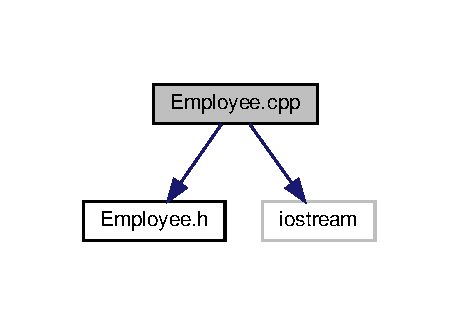
\includegraphics[width=220pt]{Employee_8cpp__incl}
\end{center}
\end{figure}


\subsection{Detailed Description}
Implementation of the \hyperlink{classEmployee}{Employee} class. 

\begin{DoxyAuthor}{Author}
Connor Walsh 
\end{DoxyAuthor}
\begin{DoxyDate}{Date}
2022-\/11-\/03 This file contains the implementation of the methods in the \hyperlink{classEmployee}{Employee} class. 
\end{DoxyDate}

\hypertarget{Employee_8h}{}\section{Employee.\+h File Reference}
\label{Employee_8h}\index{Employee.\+h@{Employee.\+h}}


\hyperlink{classEmployee}{Employee} header file.  


This graph shows which files directly or indirectly include this file\+:\nopagebreak
\begin{figure}[H]
\begin{center}
\leavevmode
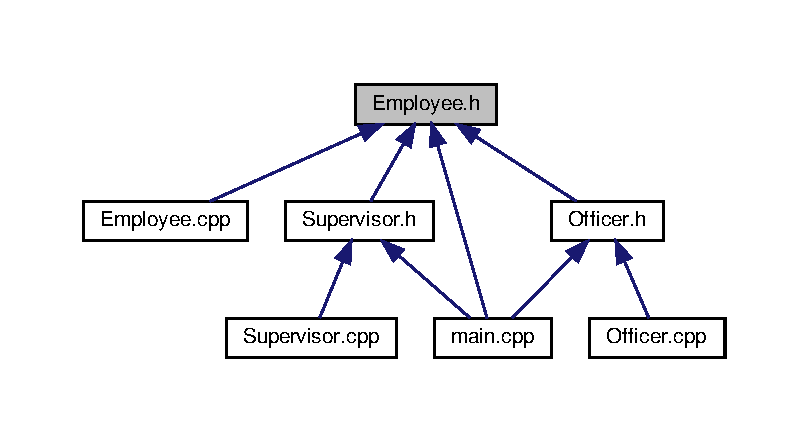
\includegraphics[width=350pt]{Employee_8h__dep__incl}
\end{center}
\end{figure}
\subsection*{Classes}
\begin{DoxyCompactItemize}
\item 
class \hyperlink{classEmployee}{Employee}
\begin{DoxyCompactList}\small\item\em This is an \hyperlink{classEmployee}{Employee} object class. \end{DoxyCompactList}\end{DoxyCompactItemize}


\subsection{Detailed Description}
\hyperlink{classEmployee}{Employee} header file. 

\begin{DoxyAuthor}{Author}
Connor Walsh 
\end{DoxyAuthor}
\begin{DoxyDate}{Date}
2022-\/11-\/03 This header file contains the definition of the \hyperlink{classEmployee}{Employee} class. 
\end{DoxyDate}

\hypertarget{main_8cpp}{}\section{main.\+cpp File Reference}
\label{main_8cpp}\index{main.\+cpp@{main.\+cpp}}


driver for the employee, supervisor, and officer classes  


{\ttfamily \#include $<$iostream$>$}\newline
{\ttfamily \#include \char`\"{}Employee.\+h\char`\"{}}\newline
{\ttfamily \#include \char`\"{}Supervisor.\+h\char`\"{}}\newline
{\ttfamily \#include \char`\"{}Officer.\+h\char`\"{}}\newline
Include dependency graph for main.\+cpp\+:\nopagebreak
\begin{figure}[H]
\begin{center}
\leavevmode
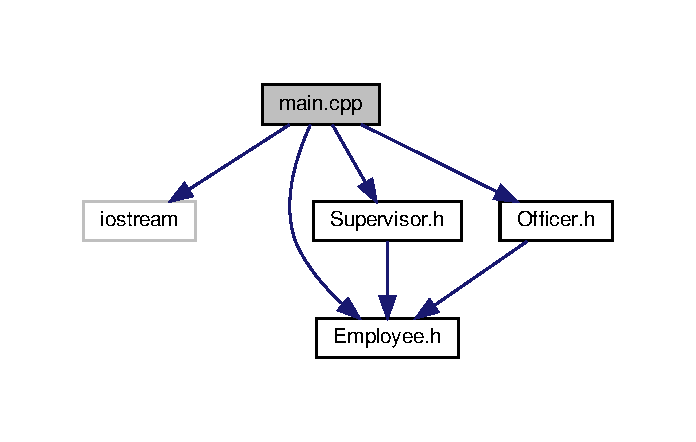
\includegraphics[width=334pt]{main_8cpp__incl}
\end{center}
\end{figure}
\subsection*{Functions}
\begin{DoxyCompactItemize}
\item 
\mbox{\Hypertarget{main_8cpp_a9ccea1912d6e2275d5612e294919d113}\label{main_8cpp_a9ccea1912d6e2275d5612e294919d113}} 
void {\bfseries run\+Employee\+Tests} (\hyperlink{classEmployee}{Employee} \&e)
\item 
\mbox{\Hypertarget{main_8cpp_ae66f6b31b5ad750f1fe042a706a4e3d4}\label{main_8cpp_ae66f6b31b5ad750f1fe042a706a4e3d4}} 
int {\bfseries main} ()
\end{DoxyCompactItemize}


\subsection{Detailed Description}
driver for the employee, supervisor, and officer classes 

\begin{DoxyAuthor}{Author}
Connor Walsh 
\end{DoxyAuthor}
\begin{DoxyDate}{Date}
2022-\/11-\/03 This driver program allows for the testing of the employee, supervisor and officer classes. 
\end{DoxyDate}

\hypertarget{Officer_8cpp}{}\section{Officer.\+cpp File Reference}
\label{Officer_8cpp}\index{Officer.\+cpp@{Officer.\+cpp}}


implementation of the \hyperlink{classOfficer}{Officer} class  


{\ttfamily \#include \char`\"{}Officer.\+h\char`\"{}}\newline
{\ttfamily \#include $<$iostream$>$}\newline
Include dependency graph for Officer.\+cpp\+:\nopagebreak
\begin{figure}[H]
\begin{center}
\leavevmode
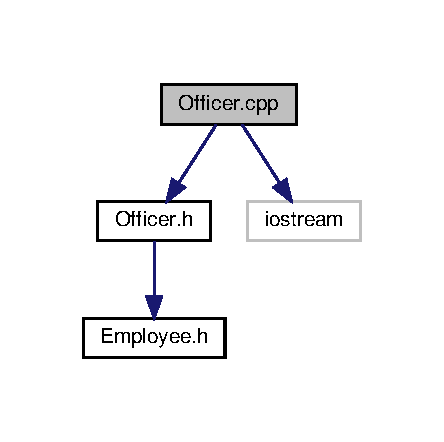
\includegraphics[width=213pt]{Officer_8cpp__incl}
\end{center}
\end{figure}


\subsection{Detailed Description}
implementation of the \hyperlink{classOfficer}{Officer} class 

\begin{DoxyAuthor}{Author}
Connor Walsh 
\end{DoxyAuthor}
\begin{DoxyDate}{Date}
2022-\/11-\/03 This file contains the implementations of the methods contained in the \hyperlink{classOfficer}{Officer} class. 
\end{DoxyDate}

\hypertarget{Officer_8h}{}\section{Officer.\+h File Reference}
\label{Officer_8h}\index{Officer.\+h@{Officer.\+h}}


Header file for the officer class.  


{\ttfamily \#include \char`\"{}Employee.\+h\char`\"{}}\newline
Include dependency graph for Officer.\+h\+:\nopagebreak
\begin{figure}[H]
\begin{center}
\leavevmode
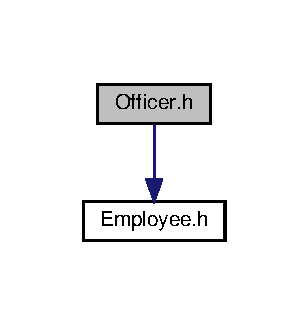
\includegraphics[width=148pt]{Officer_8h__incl}
\end{center}
\end{figure}
This graph shows which files directly or indirectly include this file\+:\nopagebreak
\begin{figure}[H]
\begin{center}
\leavevmode
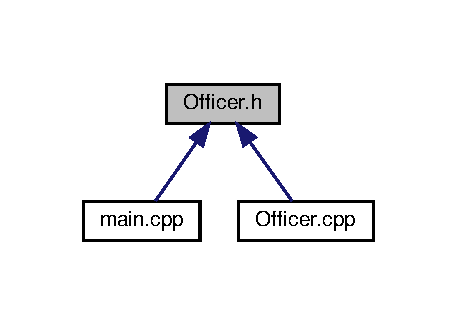
\includegraphics[width=220pt]{Officer_8h__dep__incl}
\end{center}
\end{figure}
\subsection*{Classes}
\begin{DoxyCompactItemize}
\item 
class \hyperlink{classOfficer}{Officer}
\begin{DoxyCompactList}\small\item\em class for an \hyperlink{classOfficer}{Officer} object \end{DoxyCompactList}\end{DoxyCompactItemize}


\subsection{Detailed Description}
Header file for the officer class. 

\begin{DoxyAuthor}{Author}
Connor Walsh 
\end{DoxyAuthor}
\begin{DoxyDate}{Date}
2022-\/11-\/03 This file is the definition for the officer class 
\end{DoxyDate}

\hypertarget{Supervisor_8cpp}{}\section{Supervisor.\+cpp File Reference}
\label{Supervisor_8cpp}\index{Supervisor.\+cpp@{Supervisor.\+cpp}}


implementation of the \hyperlink{classSupervisor}{Supervisor} class  


{\ttfamily \#include \char`\"{}Supervisor.\+h\char`\"{}}\newline
{\ttfamily \#include $<$iostream$>$}\newline
Include dependency graph for Supervisor.\+cpp\+:\nopagebreak
\begin{figure}[H]
\begin{center}
\leavevmode
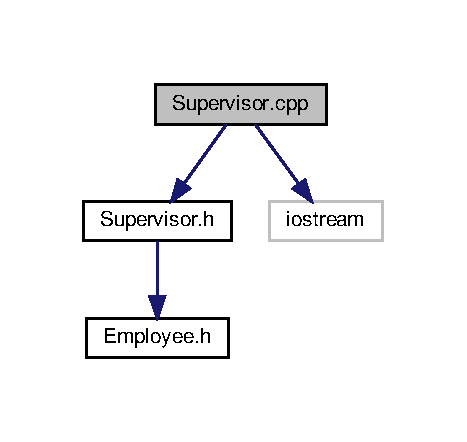
\includegraphics[width=224pt]{Supervisor_8cpp__incl}
\end{center}
\end{figure}


\subsection{Detailed Description}
implementation of the \hyperlink{classSupervisor}{Supervisor} class 

\begin{DoxyAuthor}{Author}
Connor Walsh 
\end{DoxyAuthor}
\begin{DoxyDate}{Date}
2022-\/11-\/03 This file contains the implementation of the methods in the \hyperlink{classSupervisor}{Supervisor} class. 
\end{DoxyDate}

\hypertarget{Supervisor_8h}{}\section{Supervisor.\+h File Reference}
\label{Supervisor_8h}\index{Supervisor.\+h@{Supervisor.\+h}}


\hyperlink{classSupervisor}{Supervisor} header file.  


{\ttfamily \#include \char`\"{}Employee.\+h\char`\"{}}\newline
Include dependency graph for Supervisor.\+h\+:\nopagebreak
\begin{figure}[H]
\begin{center}
\leavevmode
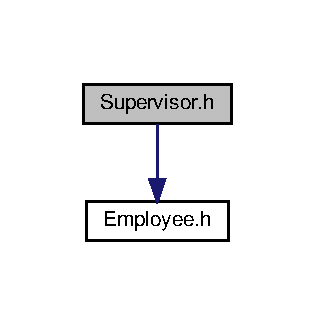
\includegraphics[width=151pt]{Supervisor_8h__incl}
\end{center}
\end{figure}
This graph shows which files directly or indirectly include this file\+:\nopagebreak
\begin{figure}[H]
\begin{center}
\leavevmode
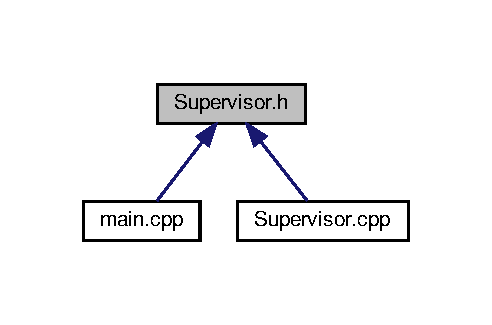
\includegraphics[width=236pt]{Supervisor_8h__dep__incl}
\end{center}
\end{figure}
\subsection*{Classes}
\begin{DoxyCompactItemize}
\item 
class \hyperlink{classSupervisor}{Supervisor}
\begin{DoxyCompactList}\small\item\em This class contains methods to store values for various \hyperlink{classSupervisor}{Supervisor} attributes. \end{DoxyCompactList}\end{DoxyCompactItemize}


\subsection{Detailed Description}
\hyperlink{classSupervisor}{Supervisor} header file. 

\begin{DoxyAuthor}{Author}
Connor Walsh 
\end{DoxyAuthor}
\begin{DoxyDate}{Date}
2022-\/11-\/03 This header file contains the definition of the \hyperlink{classSupervisor}{Supervisor} class. 
\end{DoxyDate}

%--- End generated contents ---

% Index
\backmatter
\newpage
\phantomsection
\clearemptydoublepage
\addcontentsline{toc}{chapter}{Index}
\printindex

\end{document}
